\documentclass{report}
\usepackage{graphicx}
\usepackage[round]{natbib}
%\usepackage[backend=biber]{biblatex}
%\addbibresource{bib.bib} % with extension


\begin{document}

\author{Hamid Shayestehmanesh}
\title{Exam Scheduler Application}
\maketitle
\tableofcontents
\newpage
\chapter{Introduction}
Examinations are important because they compel students to learn. Without them most students would not learn. They would learn only subjects in which they are interested and ignore the other subjects which are thought to be difficult, though they are very important in the modern age. 
\par
The way examinations are hold are very important. If they are taken very hard or very easy they cannot be trustworthy for examining and ranking students. Institutions should do their best to prepare a proper condition during exams for students so they can do their bests however, they may have limitation in resources and time.
\chapter{Goal}
Our goal in this project is to design and implement an application for scheduling exams properly. Many institutions introduces some time slots during a few days or a week to place each exam in them. For exam they will take all the exams in one week and exams can be start on 8 A.M, 11 A.M or 2 P.M. While scheduling this should be considered that a student should attend all of his/her exams and a professor should be able to be present in all of his/her exams thus, an exam should be hold in its instructor absence not two courses with same instructor should be hold in one time. These are the necessary requirement of a schedule. \par
With above information we can conclude that a student may have two exams in one day or even in contingent time slots which feels very unfair. Anyhow this should be considered that universities has different limitation based on their policies. Our goal is improving students conditions while satisfying all limitations of an institution. This soft and hard constrains will be explained completely later.

\chapter{Overview}
In this chapter we will review what is the input, output and functionality of the application and then we will review some part of the application.

\section{Input}
Information given to the system contains all the possible time slots, courses' name, students, professors and constrains. Constrains contains information about which exams can be in same day or it may bad two special exams to be held in contingent days. The details of how they are given to system are in user manual. 
% screen shot of different related parts
\section{Output}
Output is a complete schedule of exams on predefined time slots which completely satisfies all the constrains given to system. The system not only satisfies the hard constrains but also optimize soft constrains. 
% screen shot of given times
\section{Functionality}
Most important functionalities are explained as a list.
\begin{itemize}
	\item[Optimization] {Our optimization engine is the significant of the application. Our engine schedule exams in a way which all the constrains are completely satisfied and also two soft constrains are minimized.
		\subsection{constrains}
		\subsubsection{Hard Constrains}
			Hard Constrains are those which should be surely satisfied and if they cannot be, so the problem has no answer.
			\begin{itemize}
				\item{No two course of a professor are held in same time.}
				\item{Students can attend all of their exams.}
				\item{All exams will surely be hold.}
				\item{No student has two exams in a row. For example, no one will have an exam on Sunday 8 A.M and Sunday 11 A.M however, one can have exams on 8 A.M and 2 P.M.}
				\item{No two major courses of current semester will be in same day.}
			\end{itemize}
		\subsubsection{Soft Constrains}
			Soft constrains are constrains which we are trying to minimize. While minimizing these the result may not be very good or even acceptable but they are minimum and cannot be better. In such condition we should try to decrease 
			\begin{itemize}
				\item{Minimizing number of instances that a student has two exams in one day. For example if a student has two exams is Sunday it's counted as one but if a student has two exams in Sunday and two other exams in Monday then it's counted as two.}
				\item{Minimizing the number of instances that a student has two exams in contingent days. For example, a student that has a exam on Sunday and one on Saturday is counted as one.}
			\end{itemize}
			In this application we consider the first soft constrain far more important than second one therefor, first we minimize the first one and then minimize the second one. (This is not how the model is implemented but it behaves like that.)
		}
	\item[Conflict Engine] {There an engine which counts three different conflicts in a schedule. }
	\item[Manually scheduling] {Rather than scheduling automatically user can schedule exams time manually.}
\end{itemize}
\subsection{Database}
The database contains all the information we need. It's shown in the following diagram.

\centering{
	\begin{figure}
			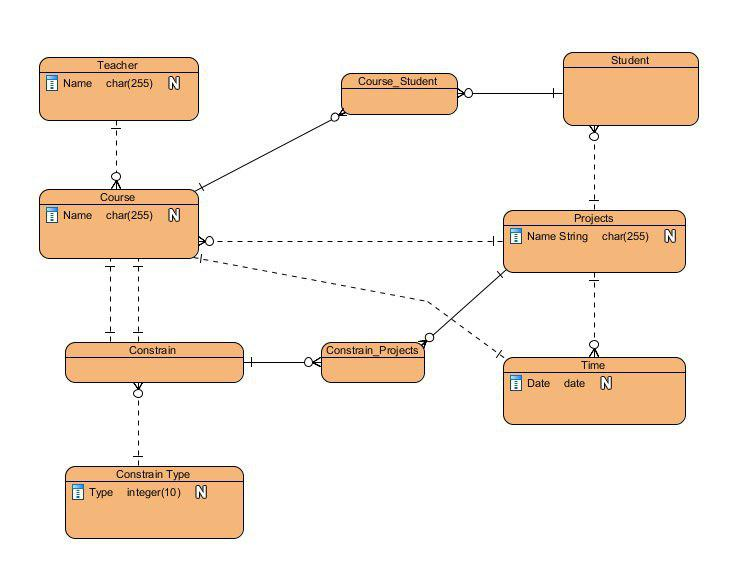
\includegraphics[width=4in]{db.jpg}
			\caption{Database ERD}
	\end{figure}

	}

\chapter{Optimization Linear Model}
This is the model we use to optimize our problem. $C, T$ are notated as number of courses and number of time slots.
\section{Available Tables}
These tables can be constructed from database base on some rules.
\begin{itemize}
\item
{\textbf{Conf \big[ C \big]\big[ C \big]  \space =} \begin{tabular}{| c | c |} \hline
number of common students between class $i, j$ & if $i \neq j$ \\ \hline
0 & if $i = j$ \\ \hline
\end{tabular}}
\end{itemize}

\section{Variables}
Variables are those which should be assigned by optimization solver.
\begin{itemize}
\item
{\textbf{SD \big[ C \big]\big[ C \big]  \space =}
\begin{tabular}{| c | c |} \hline
1 & being in same day for $i \neq j$ \\ \hline
0 & not being in same day \\ \hline
\end{tabular}}

\item{
\textbf{FS \big[ C \big]\big[ C \big]  \space =}
\begin{tabular}{| c | c |} \hline
1 & being in contingents days for $i \neq j$ \\ \hline
0 & not being in contingents day \\ \hline
\end{tabular}}

\item{
\textbf{CT \big[ C \big]\big[ T \big]  \space =}
\begin{tabular}{| c | c |} \hline
1 & if Course $c_1$ is decided to be in time $t1$  \\ \hline
0 & if Course $c_1$ is decided not to be in time $t1$ \\ \hline
\end{tabular}}


\end{itemize}

\section{Model}
\subsection{Objective}

\textbf{ \textit{Min:} } $\Sigma_{c_1}^{C} \Sigma_{c_2}^{C} SD[c_1][c_2] \times BIGM9 \times conf[c_1][c_2] + \Sigma_{c_1}^{C} \Sigma_{c_2}^{C} FD[c_1][c_2] \times BIGM6 \times conf[c_1][c_2]  $  \newline 

$BIGM9 and BIGM6$ are two big numbers which indicates the importance of each variable in our objective.
\subsection{Constraints and Explanations}

\begin{itemize}
\item{$\forall C$ \space $\Sigma_t^T CT_{ct} = 1$ \newline 
Exactly one time has been assign to each exam.}

\item{$\forall c_1 , c_2 , t $ \space if $c_1$, $c_2$ has conflicts $CT_{c_1 t} + CT_{c_2 t} \le 1$
	\newline 
	It assures that if two courses have common students or any other type of conflicts (same professor or any other type of conflicts based on policies) those won't be on same time.
	 }

\item{$\forall c_1 , c_2 , t_1 , t_2$ \space if $c_1$, $c_2$ has conflicts and $t_1, t_2$ are contingents times in a day. $$CT_{c_1 t_1} + CT_{c_2 t_2} \le 1$$ $$CT_{c_2 t_1} + CT_{c_1 t_2} \le 1 $$ 
	}

\item{$\forall c_1 , c_2 , t_1, t_2 $ \space if $c_1$, $c_2$ has conflicts and $t_1 ,t_2 $ are in same day $$CT_{c_1 t_1} + CT_{c_2 t_2} \le 1 + SD[c_1][c_2]$$ 
$$CT_{c_1 t_2} + CT_{c_2 t_1} \le 1 + SD[c_1][c_2]$$}


\item{$\forall c_1 ,  c_2 ,  t_1 , t_2$ \space if $c_1$, $c_2$ has conflicts and $t_1 , t_2$ are contingents days $$CT_{c_1 t_1} + CT_{c_2 t_2} \le 1 + FD[c_1][c_2]$$ $$CT_{c_2 t_1} + CT_{c_1 t_2} \le 1 + FD[c_1][c_2]$$  }

\end{itemize}
\section{Explanation}
FD and SD tables help us to calculate our objective cost.
\chapter{Manual}
Due to the fact that mother tongue of our application users is Farsi, the user manual is written in another document in Farsi.

\end{document}